\section{Numerik}
\subsection{Diskretisierung}
\subsubsection{1.Ableitung}

$$g'\approx \frac{g(x+\Delta x)-g(x)}{\Delta x} \qquad\qquad \text{oder} \qquad\qquad g'\approx \frac{g(x+\Delta x)-g(x-\Delta x)}{2\Delta x}\qquad \text{(Bessere Qualit�t)}$$
\subsubsection{2.Ableitung}

$g''\approx \frac{g(x+\Delta x)-2 g(x) + g(x- \Delta x)}{\Delta x^2}$

\subsection{FDM}
\textbf{TIPP:} Bei Anfangsbedingungen ungleich Null das Gleichungssystem selber von Hand herleiten, reduziert die Chance auf Fehler.
\subsubsection{Grundgleichung: $-u''(x)=f(x)$}
$ A^{(n)} \tilde{u}^{(n)} =f^{(n)}   $\\
$A^{(n)}= \frac{1}{\Delta x^2} tridiag {n-1} (-1,2,-1) = \frac{1}{\Delta x^2}
  \begin{bmatrix}
             2& -1 & 0 & \ldots \\
             -1& 2 & -1 & \ldots \\
              0& -1 & 2 & \ldots \\
              0& 0 & -1 & \ldots \\
             \ldots 
           \end{bmatrix} (eine (n-1)x(n-1)-Matrix)$\\ 
Randwert: $\tilde{u}(0)= a; \tilde{u}(n)=b $
$A^{(n)}=\tilde{u}^{(n)} =\begin{bmatrix}
             f(0) + \tilde{u}(0) \\
             f(1) \\
             \vdots  \\
             f(n) + \tilde{u}(n)
           \end{bmatrix} $\\
\subsubsection{Grundgleichung: $T''(x) + h (T_A -T(x)) = 0)$}
$-T'' + h T(x) = h T_A$\\
$A^{(n)}= \frac{1}{\Delta x^2} tridiag {n-1}
(2+h\Delta x^2 ) = \frac{1}{\Delta x^2}
  \begin{bmatrix}
             2+h\Delta x^2& -1 & 0 & \ldots \\
             -1& 2+h\Delta x^2 & -1 & \ldots \\
              0& -1 & 2+h\Delta x^2 & \ldots \\
              0& 0 & -1 & \ldots \\
             \ldots 
           \end{bmatrix} $\\       
           
           
           
\subsection{Konvergenz}
Ein Modell ist konvergent wenn bei $n\leftarrow\infty$ die Sch�tzung $\tilde{u}$ und $u$ �bereinstimmt.\\

$\boxed{||v||_{\Delta x}=\sqrt{\Delta x (v_1^2+v_2^2 + \ldots v_{n-1}^2)}= \sqrt{\Delta
x}||v||}$\\
Es konvertiert wenn: $\lim\limits_{n\to \infty
}||\tilde{u}^{(n)}-u^{(n)}||=0=\sqrt{\frac{1}{n}}||\tilde{u}^{(n)}-u^{(n)}=\sqrt{\frac{1}{n}}\sqrt{(\tilde{u}_1)-u_1)^2
+ \ldots + \tilde{u}_{n-1}-u_{n-1}}$\\

\subsection{Konsistenz}
Ein Modell ist nicht konsistent wenn das Modell durch Vereinfachung nicht mehr mit der Realit�t �bereinstimmt.

Globaler Konsistenzfehler: $\boxed{||r^{(n)}||_{1/n}\leq \frac 1{12}\max\limits_{\xi\in[0,1]}|f''(\xi)|\cdot \Delta x^2}$

\subsubsection{Residuum}
Exakt: $A^{(n)}\cdot \tilde{u}^{(n)}-f^{(n)}=0$\\
Residuum: $A^{(n)}\cdot (u^{(n)}-\tilde{u}^{(n)})=r^{(n)}$

Eine Approximationsverfahren ist Konsistent, wenn $\boxed{\lim\limits_{n\rightarrow \infty}||r^{(n)}||_{1/n}=0}$ gilt.\\

Konsistenz ist eine notwendige, aber nicht hinreichende Bedingung f�r die Konvergenz eines Verfahrens.

\subsubsection{Taylor}
$g(x)= \sum\limits_{k=0}^n\frac{1}{k!} g^{(n)}(x_0)(x-x_0)^k +
\frac{1}{(n+1)!}g^{(n+1)}(\xi)(x-x_0)^{n+1}$ = Taylor
Approximationspolynom  + Lagronesche Restglied ($\xi$ ist unabh�ngig von $x,
x_0$)



\subsubsection{Vorw�rt/R�ckw�rtsdifferenz}
$g'(x) - \frac{g(x+\Delta x) + g(x)}{\Delta x}= O(\Delta x) = 
\frac{g''(\xi_1)}{2}\Delta x^2 \Rightarrow 1.Ordnung$


\subsubsection{Zentraldifferenz}
$g'(x) - \frac{g(x+\Delta x) + g(x-\Delta x)}{2\Delta x}= O(\Delta x^2) = 
\frac{g''(\xi_1)}{2}\Delta x^2 \Rightarrow 2.Ordnung$ 



\subsubsection{2.Ableitung}
$g''(x) - \frac{g(x+\Delta x) -2 g(x)+ g(x-\Delta x)}{2\Delta x}= O(\Delta x^2)
= \frac{g''(\xi_1)}{2}\Delta x^2 \Rightarrow 1.Ordnung$

\subsection{Stabilit�t}
Die Stabilit�t einer Matrize kann �ber deren Norm $||A||_*$ bestimmt werden.\\

Es gilt: $||A||_*=\max\limits_{||X||_*=1}||A\cdot x||_*$\qquad$||A\cdot x||_*\leq||A||~||x||_*$\\

Ein Approximationsverfahren ist stabil wenn, wenn unabh�ngig von der konstante $C$ gilt:
$\boxed{||{A^{(n)}}^{-1}||\leq C}$\\



Die Bestimmung von $||A||$ ist im Allgemeinen nicht einfach, darum wird $||A||$ oft �ber den Umweg der Diagonalisierung von A bestimmt.

$y=A\cdot x\qquad\Rightarrow\qquad\tilde{y}=D\cdot\tilde{x}$\qquad mit\qquad $D=\begin{bmatrix}\lambda_1&&\\&\ddots&\\&&\lambda_n\end{bmatrix}$\\

Es gilt $TAT^T=D$, wobei T die Transformationsmatrix vom $x$-Koordinatensystem zum $\tilde{x}$-Koordinatensystem darstellt. $T$ ist orthogonal.
Die Diagonalelemente $\lambda_1,\ldots,\lambda_n$ werden auch Eigenwerte genannt.\\

Eine Approximationsformel ist stabil wenn: $\boxed{||A||=\max\limits_{k}|y_k|\leq C}$\\

Eigenwerte bestimmen: $\boxed{\det(A-\lambda I)=0}\qquad \Rightarrow \qquad \lambda_1,\ldots,\lambda_n$\\
Eigenvektoren bestimmen (f�r jedes $\lambda_i$): $A-\lambda_i I=0\qquad \Rightarrow \qquad v_1,\ldots,v_n$\\

\subsection{FDM f�r elliptisch PDGL (Poisson: $\Delta u = f$)}
%Dirichletsche Randbedingung ($u(x,y)= f(x,y) \forall (x,y)\epsilon \delta G)$\\

Gleichung:    $-\Delta u(x,y)= f(x,y) $
$\frac{g(x+\Delta x,y ) -2 g(x,y)+ g(x-\Delta x,y)}{2\Delta x} +
\frac{g(x,y+\Delta y) -2 g(x,y)+ g(x,y-\Delta y)}{2\Delta y}$\\

$h=\Delta x = \Delta y \Rightarrow \boxed{\frac 1 {h^2} (\tilde{u}_{j,k+1} +
\tilde{u}_{j+1,k} + \tilde{u}_{j,k-1} + \tilde{u}_{j-1,k} - 4 \tilde{u}_{j,k})
= f_{j, k}}$\\[0.4cm]


$B \tilde{u} = f \Rightarrow B= \begin{bmatrix}
             T& D & 0 & \ldots \\
             D& T & D & \ldots \\
              0& D & T & \ldots \\
              0& 0 & D & \ldots \\
             \ldots 
           \end{bmatrix}$
wobei $T=\begin{bmatrix}
             4& -1 & 0 & \ldots \\
             -1& 4 & -1 & \ldots \\
              0& -1 & 4 & \ldots \\
              0& 0 & -1 & \ldots \\
             \ldots 
           \end{bmatrix}$
und $D=\begin{bmatrix}
             -1& 0& 0 & \ldots \\
             0 & -1 &  & \ldots \\
              0& 0&-1 & \ldots \\
             \ldots 
           \end{bmatrix}$

           
\subsubsection{Irregul�re Gitter (f�r den Rand)}
\begin{minipage}{5cm}
	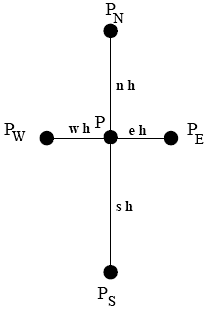
\includegraphics[width=5cm]{Content/Numerik/irregulaereGitter.png}

\end{minipage}
\begin{minipage}{14cm}

$\left(\frac{u(x+eh,y)-u(x,y)}{e(e+w)} +\frac{u(x+wh,y)-u(x,y)}{w(e+w)}+\frac{u(x+nh,y)-u(x,y)}{n(n+s)} + \frac{u(x+sh,y)-u(x,y)}{n(n+s)}\right)\frac{2}{h^2}=f(x,y)$\\

oder
\\

$\frac{u(P_E) - u(P)}{e(e+w)} + \frac{u(P_W) - u(P)}{w(e+w)} + \frac{u(P_N) - u(P)}{n(n+s)} + \frac{u(P_S) - u(P)}{s(n+s)} = \frac{h^2}{2} f(x,y)$
\end{minipage}
\subsubsection{Neumann Rand 
%$\partial_n u(x,y) \forall (x,y) \epsilon \partial_n G$
}
\begin{minipage}{8cm}
	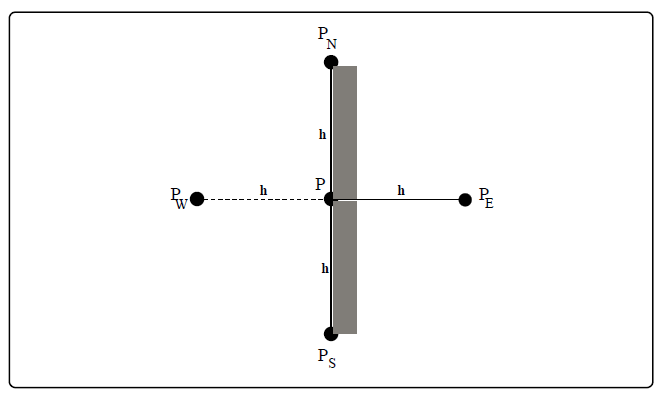
\includegraphics[width=8cm]{Content/Numerik/NeumannRand.png}


\end{minipage}
\begin{minipage}{10cm}
In einem Randpunkt P liegen wie in der Abbildung ersichtlich, $P_N$ und $P_S$ auf dem Rand von Omega, $P_W$ liegt ausserhalb von Omega.\\
In P sei die Neumannsche Randbedingung: $\boxed{\partFrac{u}{n}(P)=g(P)}$\\
$u_x(P)=\frac{u(P_E)-u(P_W)}{2h}\quad\Rightarrow\quad u(P_W)=u(P_E)-2h\cdot u_x(P)$\\

$\boxed{\frac{2u(P_E) + u(P_N) +
u(P_S)- 4 u(P) - 2h\cdot u_x(P)}{h^2}}$\\


\textbf{Spiegelmethode}:\\
Wenn $u_x(x,y) = 0$, dann spricht man auch von der Spiegelmethode. Die Punkte $P_W$ und $P_E$ weisen dann die gleiche Wertigkeit auf ($P_W=P_E$).
\end{minipage}


\subsection{FDM f�r parabolische PDGL}
\subsubsection{Explizites Verfahren (Richardson-Verfahren)}
$$\frac{u(x,t+\Delta t) - u(x,t)}{\Delta t} = 
\frac{u(x+\Delta x, t)-2u(x,y) + u( x - \Delta x, t )} {\Delta x^2} $$ 
$$\delta_t
u(x,t)=\delta_{xx}(x,t)$$ 
$ u_{j,k+1} = r \tilde{u}_{j-1,k} + (1-2r)\tilde{u}_{j,k} + r \tilde{u}_{j+1,k}
\Longrightarrow$ aus den Positionen k wird k+1 berechtet $r=\frac{\Delta
t}{\Delta x^2}$

\subsubsubsection{LinAlg-Ansatz}: 
F�r Dimensionen: $n = \lceil\frac{x_{max} - x_{min}}{\Delta x}\rceil$. 
Initialwerte: $\underline{\tilde{u}}^{(0)} = f(x,0)$ mit $x \in \{\Delta x, \dots, (n-1) \Delta x\}$ ($n-1 \times 1$ Vektor). 
$C = \operatorname{tridiag}_{n-1}(r, 1-2r, r)$ ($n-1 \times n-1$ Matrix). Iterative Berechnung: $\underline{\tilde{u}}^{(k+1)} = C \underline{\tilde{u}}^{(k)}$
Absolute Berechnung: $\underline{\tilde{u}}^{(k)} = C^k \underline{\tilde{u}}^{(0)}$

Nachteil:\\
$$||A^{-1}|| < 1 \Longrightarrow \text{um stabiles Verfahren muss} r <
\frac{1}{2}$$

\subsubsection{Implizites Verfahren}
Im Unterschied zum expliziten Verfahren, das Werte vom vorherigen Zeitpunkt nutzt, wird hier das ein Gleichungssystem global gel�st.
$$\frac{u(x,t) - u(x,t -\Delta t)}{\Delta t} = 
\frac{u(x+\Delta x, t)-2u(x,y) + u( x - \Delta x, t )} {\Delta x^2} $$ 
$ u_{j,k} = r \tilde{u}_{j-1,k+1} + (1+2r)\tilde{u}_{j,k+1} + r \tilde{u}_{j+1,k+1}
\Longrightarrow
u^{(k)} = E^{(n)} u^{(k+1)}$ Da $||(E^{(n)})^{-1}|| $ immer $< 1$ konvergiert
das implizite Verfahren immer.

\todo{Das wichtigste steht nicht: $E^(n)$!!}

\subsubsection{Crank Nicolson -Verfahren (explizite + implizite Verfahren)}


$$ r \tilde{u}_{j-1,k+1} + (2+2r)\tilde{u}_{j,k+1} + r \tilde{u}_{j+1,k+1} = r
\tilde{u}_{j-1,k+1} + (2-2r)\tilde{u}_{j,k+1} + r \tilde{u}_{j+1,k+1} $$

$$
  \begin{bmatrix}
             2-2r& r & 0 & 0\\
             r & 2-2r & r & 0  \\
              0& r &2-2r& r  \\
              0& 0 & r &2-2r \\
             \ldots 
           \end{bmatrix} 
  \begin{bmatrix}
  	T_{1,0}\\
  	T_{2,0}\\
  	T_{3,0}\\
  	T_{4,0}\\
  \end{bmatrix} +
  \begin{bmatrix}
  	T_{0} r\\
  	0\\
  	0\\
  	T_{L} r\\
  \end{bmatrix} = 
  \begin{bmatrix}
             2+2r& -r & 0 & 0\\
             -r & 2+2r & -r & 0  \\
              0& -r &2+2r& -r  \\
              0& 0 & -r &2+2r \\
             \ldots 
           \end{bmatrix} 
  \begin{bmatrix}
  	T_{1,1}\\
  	T_{2,1}\\
  	T_{3,1}\\
  	T_{4,1}\\
  \end{bmatrix} -
  \begin{bmatrix}
  	T_{0} r\\
  	0\\
  	0\\
  	T_{L} r\\
  \end{bmatrix}
  $$
  $\Longrightarrow G^{(n)} u^{(k)} = F^{(n)} u^{(k+1)} \Longrightarrow
  u^{(k+1)}= (F^{(n)})^{-1} G^{(n)} u^{(k)}$

  
  
  
 
\subsection{FDM f�r Hyperbolische PDGL}

$$u_{tt}=u_{xx} = homogen$$
$$u_{tt} -u_{xx}= v(x,t) = inhomogen$$

$$\Longrightarrow u_{j,k+1}=r^2 u_{j-1,k} 2(1-r^2)u_{j,k}+ r^2
u_{j+1,k}-u_{j,k-1}$$
\subsubsection{Anfangsbedingungen}
$$\tilde{u}_{j,0} = f(j\Delta x); u_{j,1}= f(j\Delta x) + g(j\Delta x)\Delta t$$
(f(x)= Anfangsfunktion; g(x)=Ableitung; $r = \frac{\Delta t}{\Delta x}$)

\subsubsection{Transportgleichung}
$$u_x(x,t) + u_t(x, t) = 0; u(x,0)=P(x-t)$$
$$\frac{u(x,t+\Delta t)-u(x,t)}{\Delta t} = \frac{u(x,t) - u(x-\Delta x,
t)}{\Delta x}$$
